\documentclass{tufte-handout}
\usepackage{braph2_tut}
%\geometry{showframe} % display margins for debugging page layout

\title{Brain Atlas}

\author[The BRAPH~2 Developers]{The BRAPH~2 Developers}

\begin{document}

\maketitle
	
\fig{marginfigure}
	{fig:01}
	{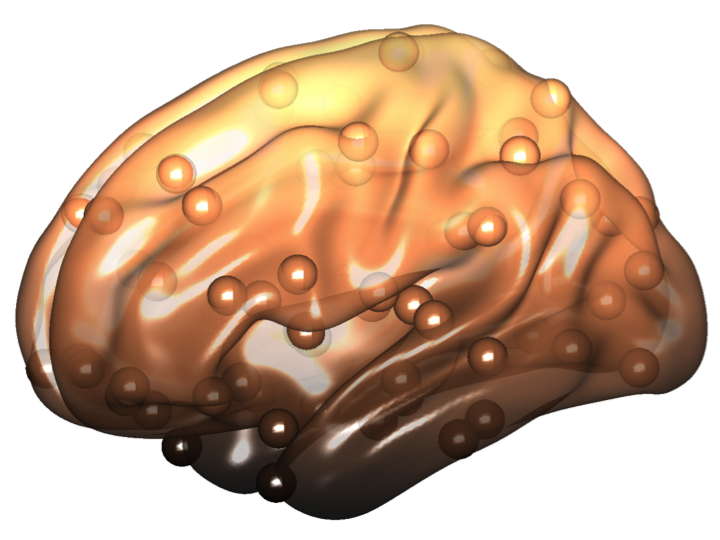
\includegraphics{tut_ba/fig1.png}}
	{Brain regions.}
	{
	Image with a brain surface and some brain regions.
	}

\begin{abstract}
\noindent
This is the tutorial to work with the Graphical User Interface (GUI) to manage brain atlases, which is typically the first step that is required to perform a graph analysis in BRAPH 2.0. 
In this Tutorial, we will explain you how to upload a brain atlas and how to visualize it.
\end{abstract}

\tableofcontents

\fig{figure*}
	{fig:02}
	{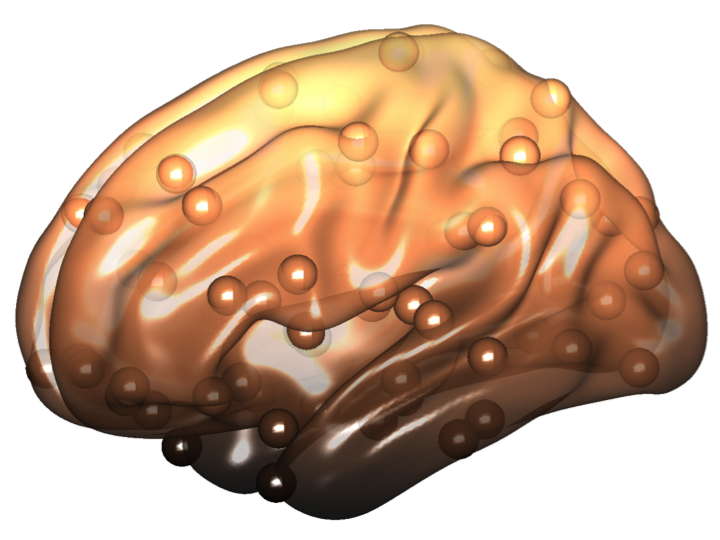
\includegraphics[height=10cm]{tut_ba/fig1.png}}
	{Brain Atlas GUI.}
	{
	Graphical user interface to work with brain atlases. 
	\textcolor{red}{Add image with full interface.}
	}

\clearpage
\section{Open the GUI}

The Brain Atlas GUI is typically the first step in the BRAPH 2.0 pipelines. You can also do it by typing braph2, which will open the Graphical User Interface of the BRAPH 2.0 software. Here you must first select a Pipeline containing the analyses steps that you want to apply to your data. Once a Pipeline has been selected, the first window will allow you to upload the Brain Atlas, as shown in \Figref{}.

To open the Graphical User Interface and Upload the Brain Atlas, you can also do it from the command line by typing the commands in \Coderef{cd:launch}.
%
\begin{lstlisting}[
	label=cd:launch,
	caption={
		{\bf Code to launch the Brain Atlas GUI.}
		This code can be used in the MatLab command line to launch the  Brain Atlas GUI.
	}
]
ba = BrainAtlas(); ¥\circled{1}\circlednote{1}{creates a new object \code{BrainAtlas}.}¥

gui = GUIElement('PE', ba); ¥\circled{2}\circlednote{2}{creates a GUI to upload the brain atlas.}¥
gui.get('DRAW') ¥\circled{3}\circlednote{3}{draws the GUI.}¥
gui.get('SHOW') ¥\circled{4}\circlednote{4}{shows the GUI.}¥
\end{lstlisting}

\fig{figure}
	{fig:xxx}
	{
	[b!]
	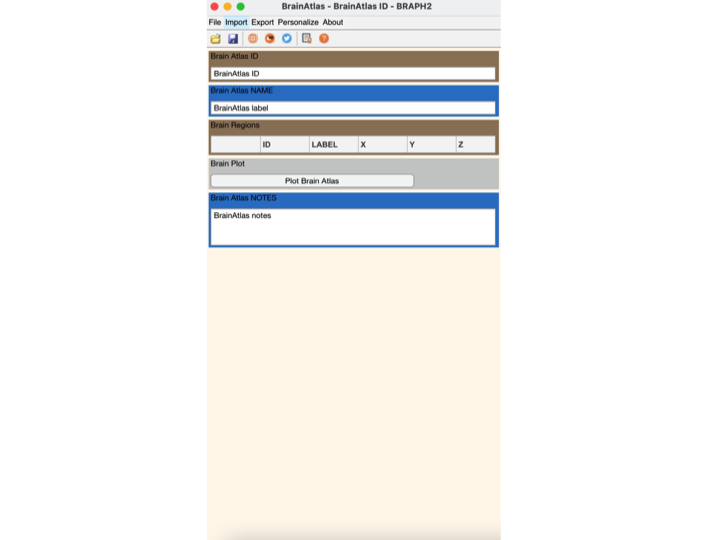
\includegraphics{tut_ba/fig7.png}
	}
	{Brain Atlas GUI.}
	{
	Graphical user interface to work with brain atlases. 
	}

\clearpage
\section{Upload the Brain Atlas}

In this window you have a Menu that you can use to Open a File (File -> Open) and select a Brain Atlas that is already prepared or Import (Import -> File) a Brain Atlas you have created in excel or text format. If you Import a Brain Atlas you have created and an error message appears, check again your Brain Atlas file for missing or incorrect information based on the format for new Brain Atlases we describe above. 
Once you have uploaded a Brain Atlas, you will notice that the information regarding the Brain Atlas ID, Brain Atlas NAME and Brain Regions sections are now filled with the information of the atlas. You can edit the information included in any of these sections. 

\fig{figure}
	{fig:xxx}
	{
	[b!]
	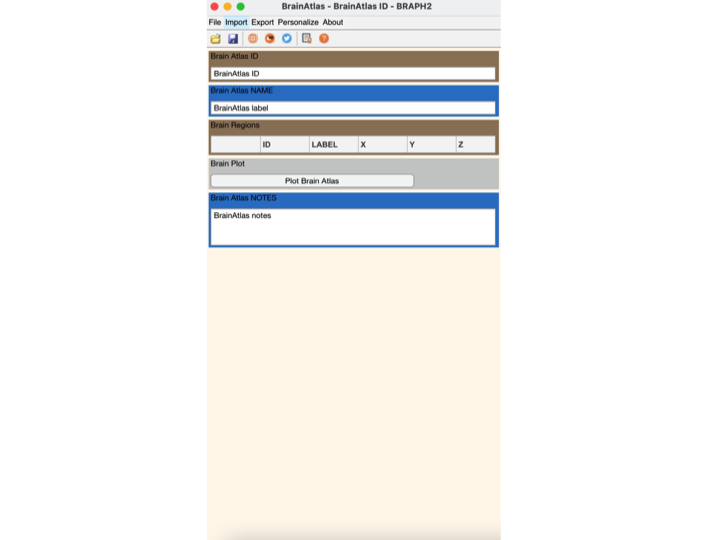
\includegraphics[height=4cm]{tut_ba/fig7.png}
	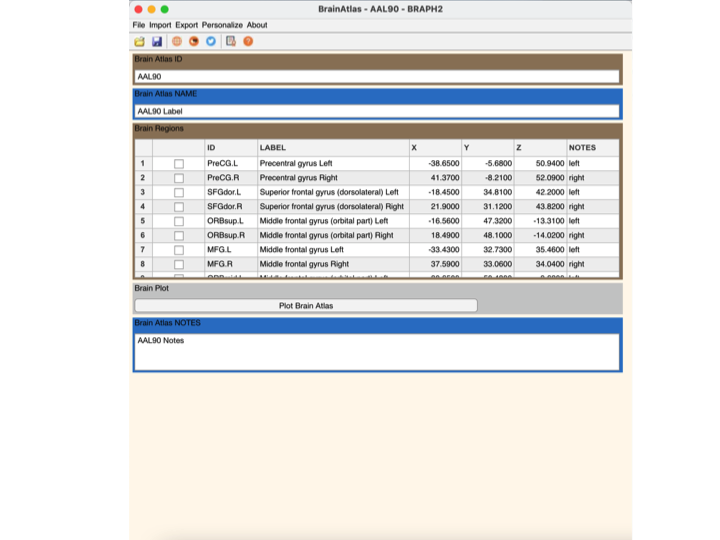
\includegraphics[height=4cm]{tut_ba/fig8.png}
	}
	{Brain Atlas GUI.}
	{
	Graphical user interface to work with brain atlases. 
	}

\clearpage
\section{Ready Brain Atlases}

\marginnote{
\begin{itemize}
\item {\bf AAL90} Automated Anatomical Labelling atlas with 90 cortical and subcortical regions.
\item {\bf AAL116} Automated Anatomical Labelling atlas with 116 cortical and subcortical regions, including cerebellar areas.
\item {\bf BNA} Brainnetome atlas with 246 cortical and subcortical regions.
\item {\bf Craddock} Functional atlas with 200 cortical and subcortical regions.
\item {\bf Desikan} Anatomical atlas with 68 cortical and 14 subcortical gray matter regions derived from the FreeSurfer software.
\item {\bf Destrieux} Anatomical atlas with 148 cortical and 14 subcortical gray matter regions derived from the FreeSurfer software.
\item {\bf Schaefer} Functional brain atlas with 200 cortical regions that belong to 7 different resting-state fMRI networks.
\end{itemize}
}

Currently, we provide several brain atlases that are commonly used in the field of brain connectomics, which can be downloaded from our website (\url{http://braph.org/software/brain-atlases/}).

\clearpage
\section{Create a New Brain Atlas}

To prepare a Brain Atlas in BRAPH 2.0 format, you should create a new excel file (.xls or .xlsx), as shown in \Figref{fig:xls}.

\fig{figure}
	{fig:xls}
	{
	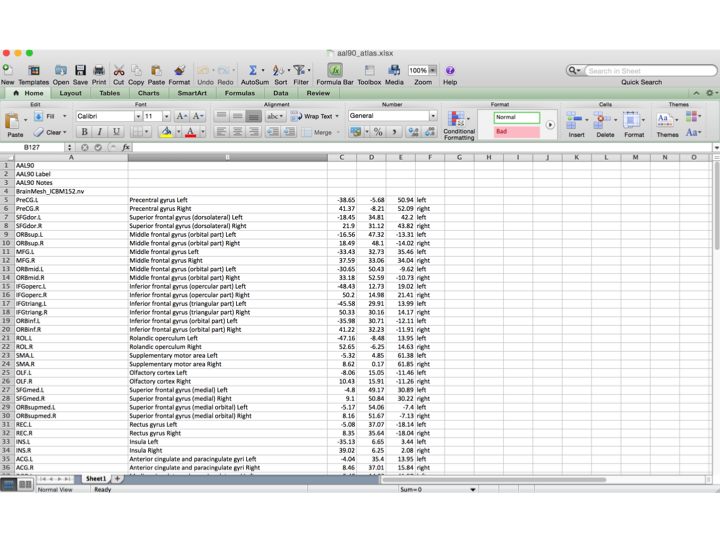
\includegraphics{tut_ba/fig9.png}
	}
	{Brain Atlas GUI.}
	{
	Graphical user interface to work with brain atlases. 
	}

Start by writing the following information in the first 4 rows:
\begin{itemize}

\item Brain Atlas ID (row 1, column 1). 
For example: Desikan FreeSurfer

\item Brain Atlas LABEL (row 2, column 1). 
For example: Desikan FreeSurfer Labels

\item Brain Atlas NOTES (row 3, column 1).
For example: Desikan FreeSurfer Nodes

\item Brain Surface Name (row 4, column 1).
For example: BrainMeshICBM152.nv

\end{itemize}
Then, from row 5, you should include the IDs of the regions of your atlas (1st column), the Labels of the regions of your atlas (2nd column), the X, Y and Z coordinates (3rd, 4th and 5th columns) and the brain hemisphere or any notes you would like to add (6th column).	

\clearpage
\section{Plot the Brain Atlas}

Once you are satisfied you can proceed with the option "Plot Brain Atlas", which will open a brain surface that contains the nodes corresponding to the regions of your atlas.

\fig{figure}
	{fig:xxx}
	{
	[b!]
	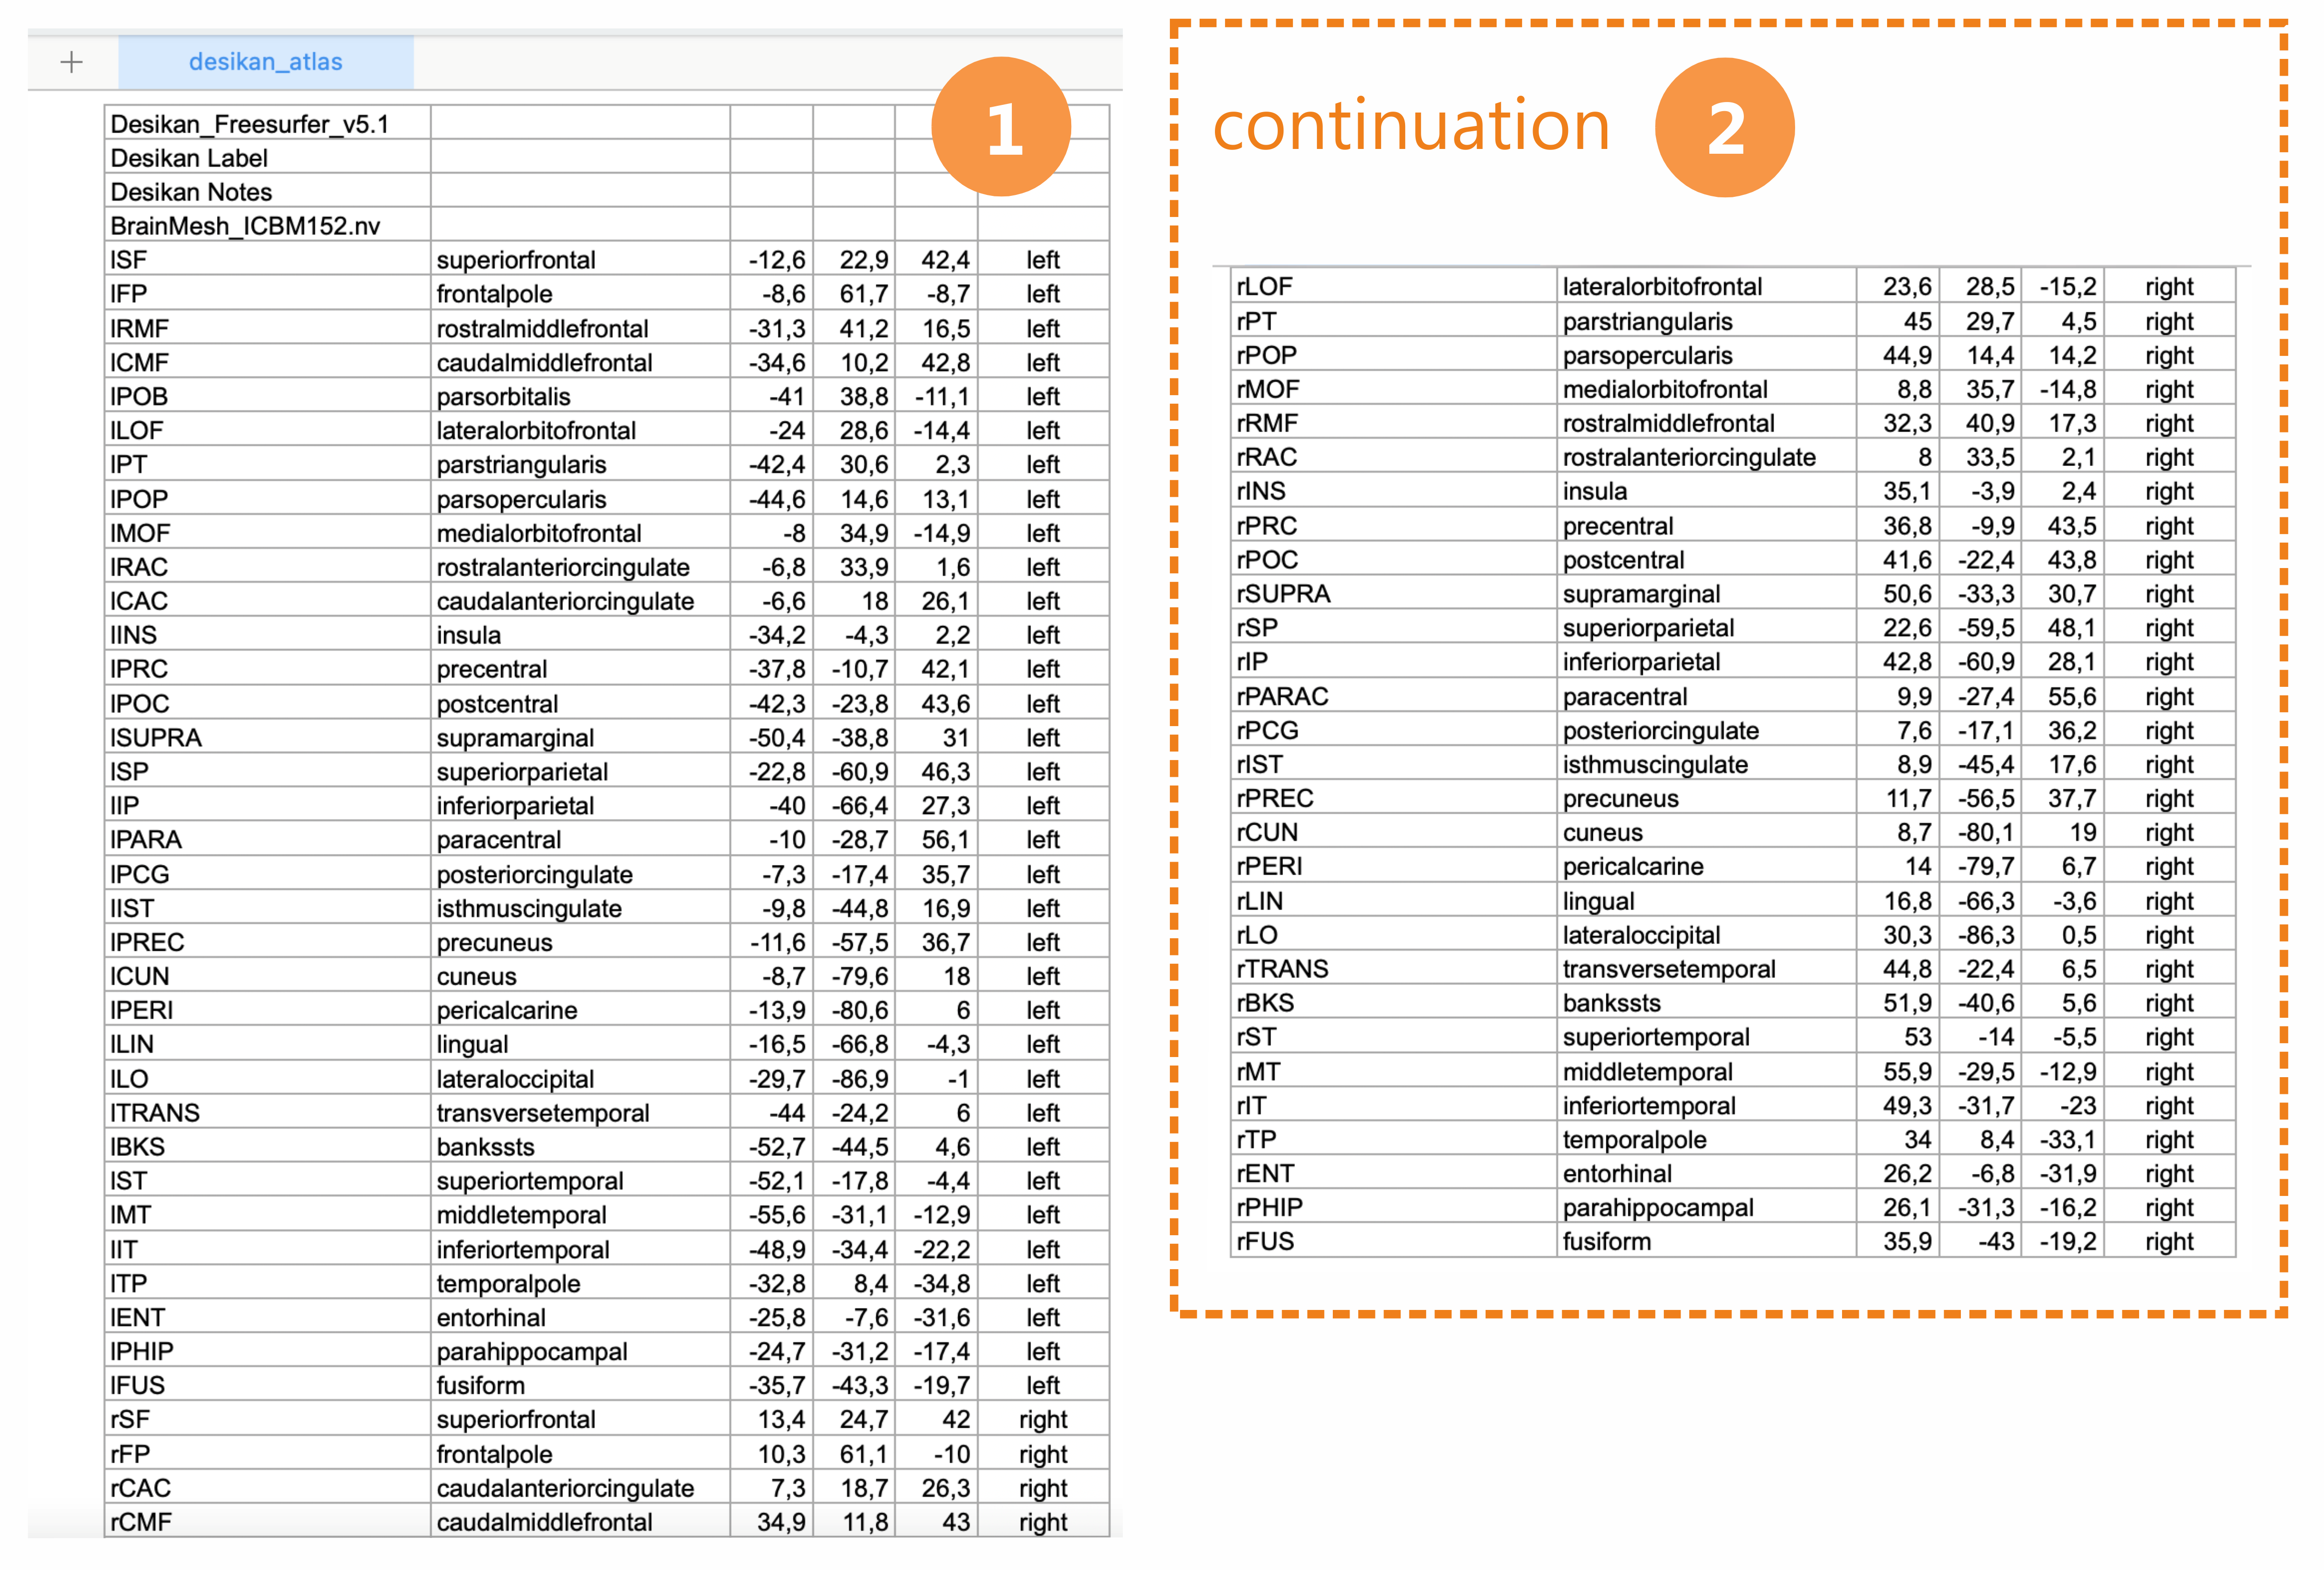
\includegraphics{tut_ba/fig2.png}
	}
	{Brain Atlas GUI.}
	{
	Graphical user interface to work with brain atlases. 
	}
This new window has a large menu that allows you to change its visualization. We suggest you try the different options to understand how they change the figure. Importantly, within this menu there is one option called Settings Brain Surface which, when selected, will open another window, as can be seen in the snapshot below:

\fig{figure*}
	{fig:xxx}
	{
	[b!]
	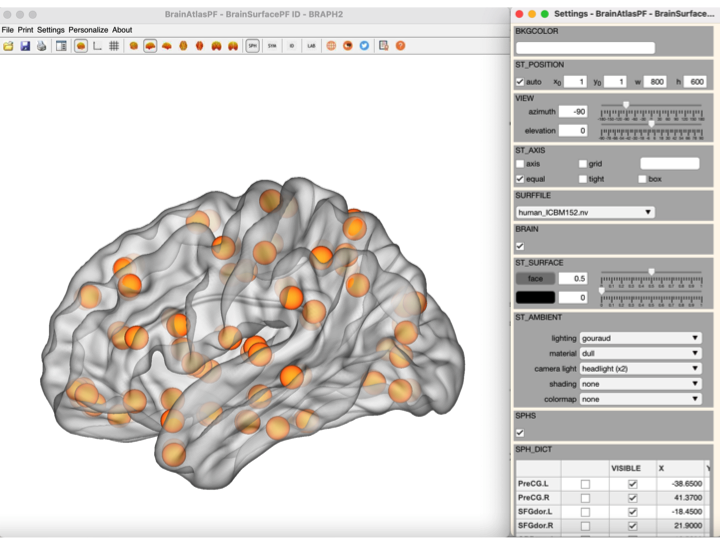
\includegraphics{tut_ba/fig3.png}
	}
	{Brain Atlas GUI.}
	{
	Graphical user interface to work with brain atlases. 
	}

This window allows you to change different visualization options, which are important to create a final figure with all the nodes included in your analysis, which is often included within the 1st Figure of a manuscript.


Most things in this panel are intuitive and again we suggest that you try different options until you achieve the visualization you desire, for example:

 \fig{figure*}
	{fig:xxx}
	{
	[b!]
	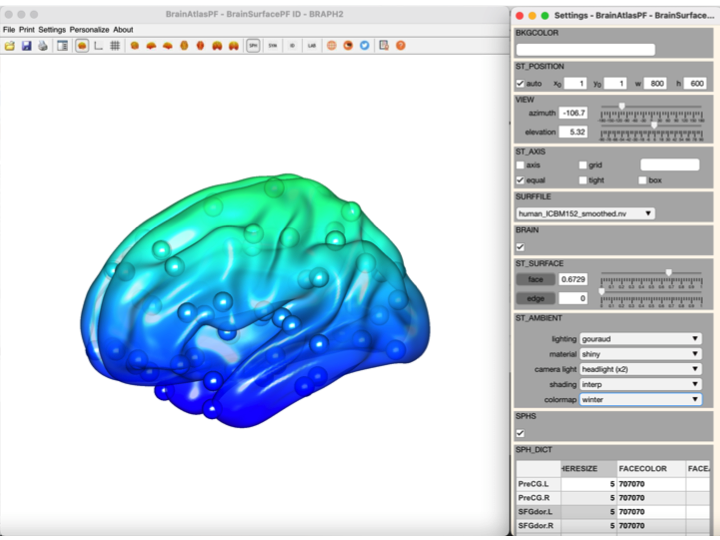
\includegraphics{tut_ba/fig4.png}
	}
	{Brain Atlas GUI.}
	{
	Graphical user interface to work with brain atlases. 
	}


Some things that might not be intuitive is the difference between spheres and symbols (the first one is the geometrical structure of a node, whereas the second is just a dot inside the sphere that denotes the presence of a region). 


If you wish to change the size of the spheres of all nodes, you need to change the size of one node, select other nodes in the first column, right click to select Apply to Selection.


Finally the codes for different colours in the FACECOLOR column correspond to the hexadecimal form of RGB colors, which can be found online.

\clearpage
\section{Export the Figure}

xxx

\end{document}